\begin{figure}[h!]
	\centering
	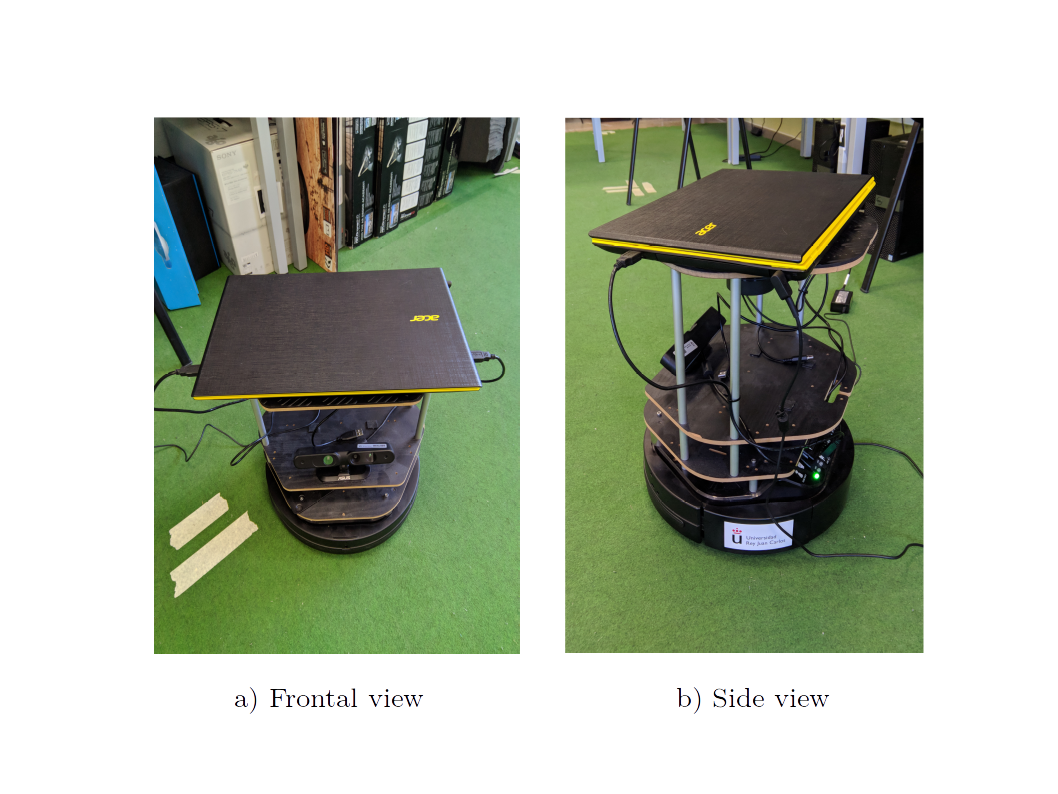
\includegraphics[width=7.5cm]{images/exp_set}
	\caption{Robot used for the validation experiments.}
	\label{fig:exp_set}
\end{figure}


\section{Experiments}
\label{sec:experiments}

The developed system has been experimentally validated on a real robot and an indoor scenario. The TurtleBot-2 robot was used on the experiments, including an Asus Xtion Pro Live RGBD sensor. The onboard computer was a regular laptop with Intel i5-4210U CPU, 8GB of RAM DDR3L and Nvidia 940M GPU (Figure \ref{fig:exp_set}). 

% \begin{figure}[h]
% 	\centering
% 	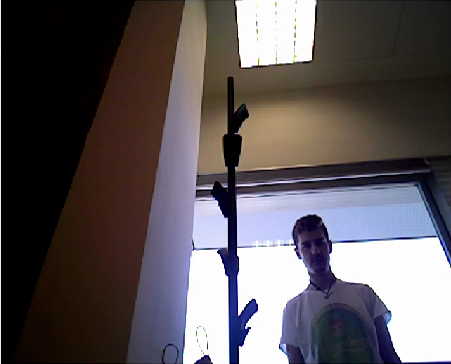
\includegraphics[width=4.5cm]{images/light_ko_2}
% 	\caption{Harsh lighting conditions.}
% 	\label{fig:exp_lighting}
% \end{figure}


The person detection and reidentification process can be observed on Fig. \ref{fig:exp_figures}. The system is succesfully able to re-identify the target person (\textit{mom}), even in challenging lightning conditions like in Figure \ref{fig:exp_figures}.

\begin{figure}[h!]
	\centering
	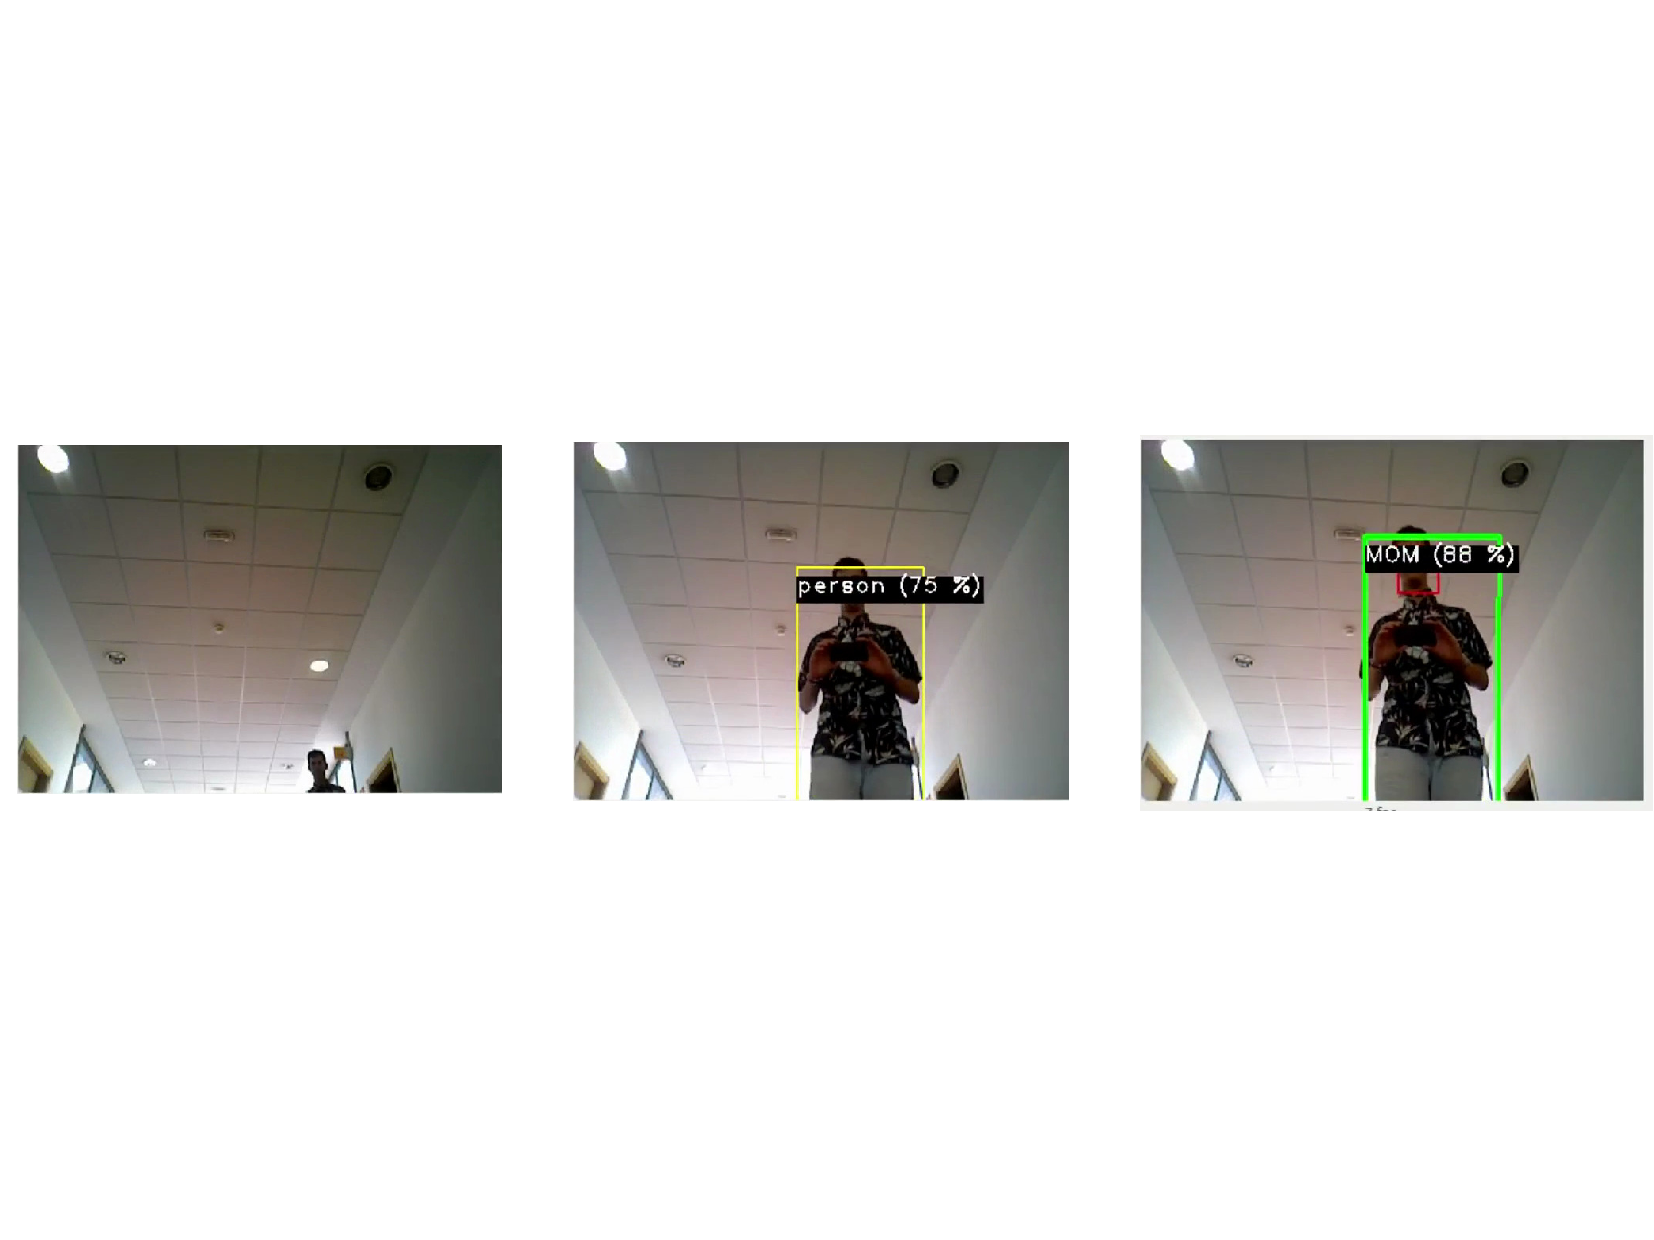
\includegraphics[width=12cm]{images/exp_tracking}
	\caption{Detection and re-identification of the target person.}
	\label{fig:exp_figures}
\end{figure}

The complete system results show a robot finely following a particular person, even when that person does not face towards the robot. The behavior is fluent, with a refresh rate of 10 movements per second (as the SSD CNN is the lightest possible model, as seen on Table \ref{tab:model_tests}). This agility of the neural network for people detection helped substantially to minimize the time bottleneck. The following behavior can be observed on Fig. \ref{fig:exp_following}. Several videos of a typical execution are also publicly available \footnote{Full video test available on \url{https://www.youtube.com/watch?v=oKMR_QCT7EE}}.

\begin{figure}[h!]
	\centering
%        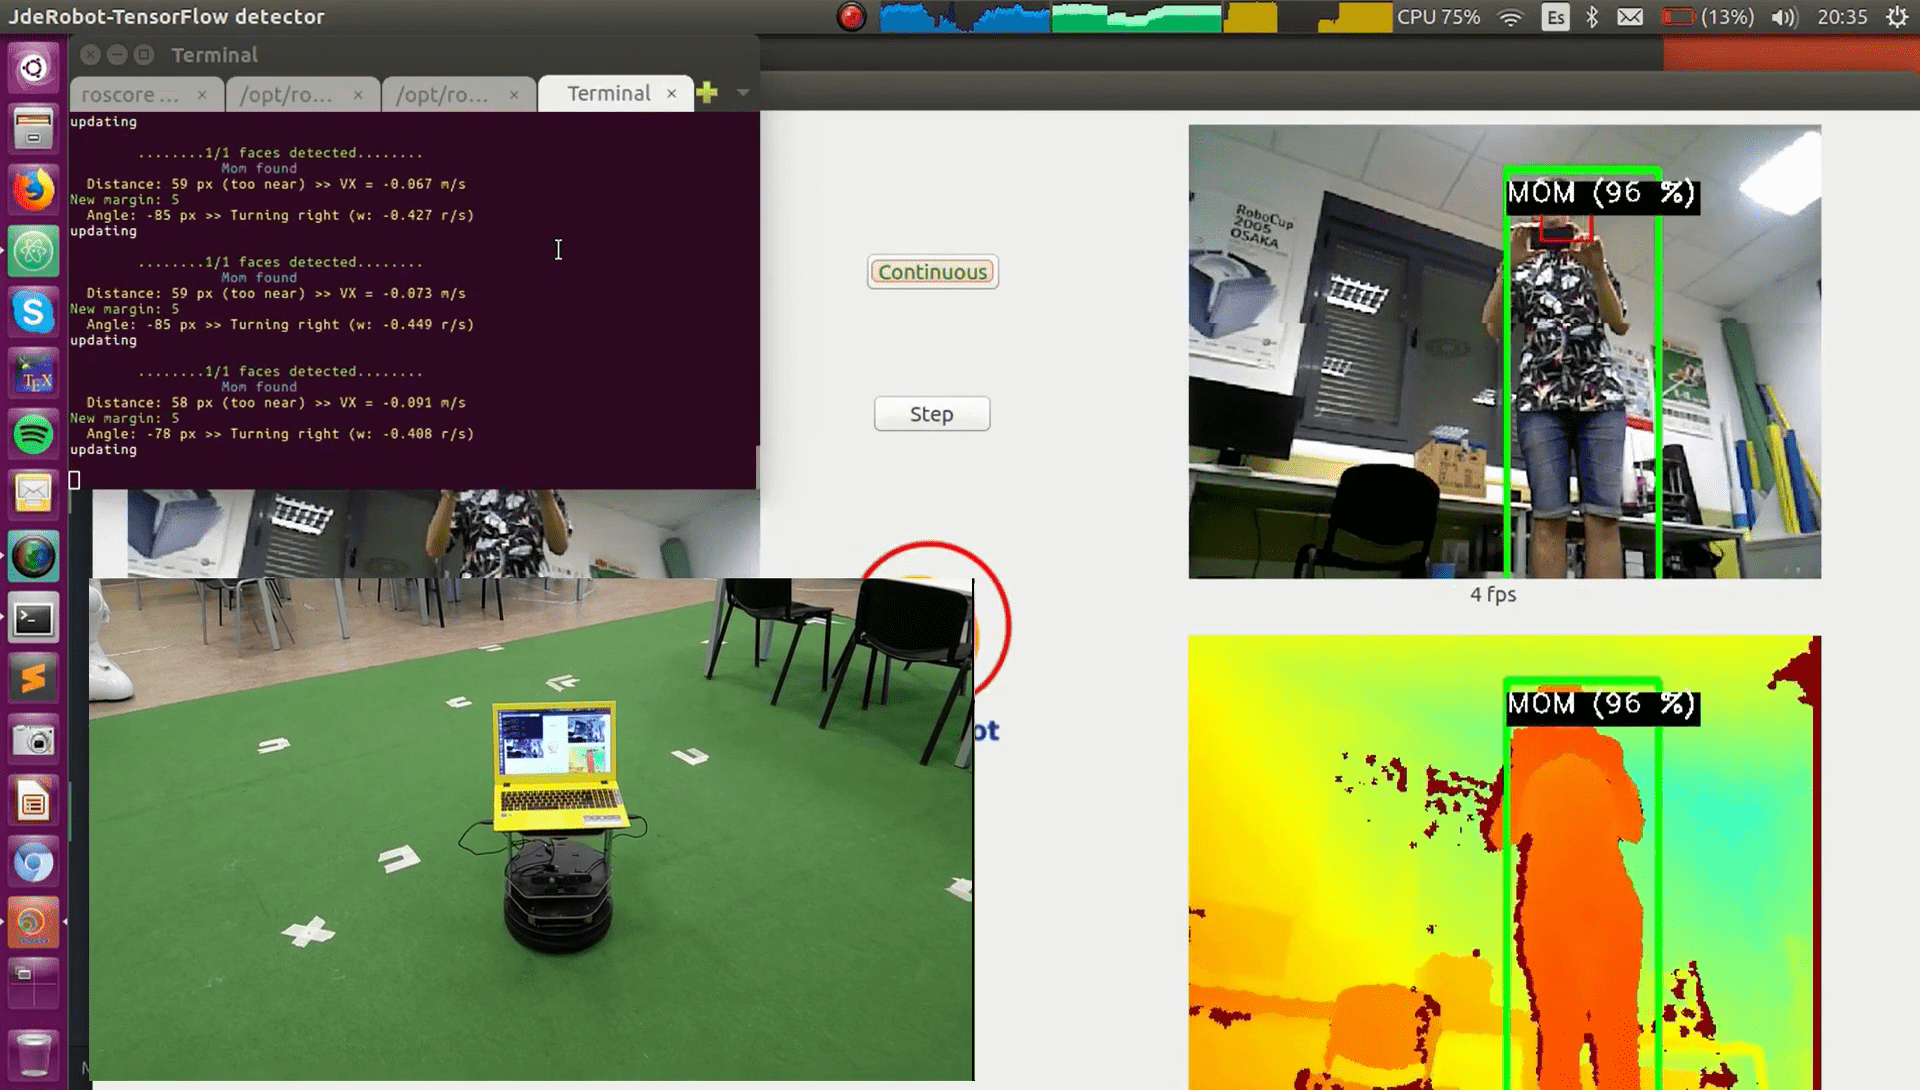
\includegraphics[width=12cm]{images/followperson_working.png}
	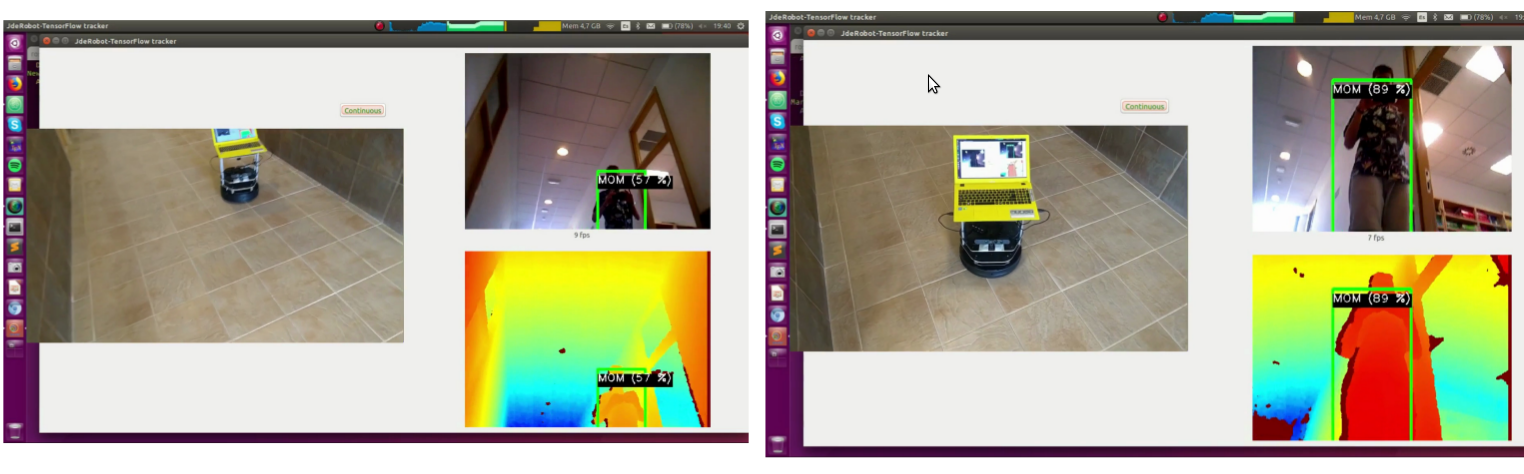
\includegraphics[width=12cm]{images/followperson_working2.png}
	\caption{Following behavior.}
	\label{fig:exp_following}
\end{figure}